\documentclass{llncs}
\usepackage{graphicx}

\usepackage{algorithm}
\usepackage{algorithmic}
\usepackage{amsmath}
\usepackage{amssymb}

\usepackage{subfigure} 
% For citations
\usepackage{natbib}

% For algorithms
\usepackage{algorithm}
\usepackage{algorithmic}
\usepackage{amsmath}
\usepackage{amssymb}

\usepackage{todonotes}
\usepackage[nomarkers, nolists]{endfloat}
\renewcommand{\efloatseparator}{\mbox{}}
\usepackage{hyperref}

% Packages hyperref and algorithmic misbehave sometimes.  We can fix
% this with the following command.
\newcommand{\theHalgorithm}{\arabic{algorithm}}
\def\code#1{\texttt{#1}}

\usepackage{caption}
\usepackage{float}
\usepackage{bbm}

%\floatname{algorithm}{Procedure}
\renewcommand{\algorithmicrequire}{\textbf{Input:}}
\renewcommand{\algorithmicensure}{\textbf{Output:}}




%\usepackage{capt-of}



\begin{document}

\title{Integrated Perception and Control at High Speed: Evaluating Collision Avoidance Maneuvers Without Maps}
\author{Pete Florence\inst{1} \and John Carter\inst{1} \and Russ Tedrake\inst{1} }
\institute{MIT Computer Science and Artificial Intelligence Laboratory, Cambridge, MA \email{\{peteflo,jcarter,russt\}@csail.mit.edu}}

\maketitle

\begin{abstract}
We present a method for robust high-speed quadrotor flight through unknown cluttered environments using a fast approximation of collision probabilities. Motivated by experiments in which the difficulty of accurate state estimation was a primary limitation on speed, our method forgoes maintaining a map in favor of using only instantaneous depth information in the local frame. This provides robustness in the presence of significant state estimate uncertainty. Additionally, we present approximation methods augmented with spatial partitioning data structures that enable low-latency, real-time reactive control. The probabilistic formulation provides a natural way to integrate reactive obstacle avoidance with arbitrary navigation objectives. We validate the method using a simulated quadrotor race through a forest at high speeds in the presence of increasing state estimate noise. We pair our method with an MPC-based motion primitive library and compare with a global path-generation and path-following approach.
\end{abstract}

%\section{Introduction}
%
%Fair amount of people have done obstacle avoidance in a local frame.  What we do is not even build a map.  If we use only the instantaneous depth information, and figure out a smart way to impose soft costs, then we won't even need a map. The question is how to do that soft cost.  The key we have found is to evaluate maneuvers and consider uncertainty.  One way to think about this method is a reactive controller that involves rigorous state-space design.  Shares the property of reactive controllers of being memoryless, and shares the property of robust planning approaches of considering uncertainty together with a state-space dynamics model. At slow speeds, it's not optimal.  Like other reactive-type approaches, it may be short-sighted at least without proper tuning.  We still think maps are important.  When dead-ends and bugtraps are involved, a reactive controller will not work, and maps are one route to solving the navigation problem.  At slower speeds, with less dynamic locomotion regimes, building maps is feasible.
%
%WIP: Sensing in service of control.   Perception's role is to validate control.  Integration of perception and control.  Planning (hard to add sensor noise) vs. Reactive (hard to add navigation objectives).  A key insight is that we can estimate the probability of collision for any action without even building a locally consistent map.  Consider local maps.  An interesting regime to think about is where we are going too fast for stopping, and we just need to swerve.

%
%
%
%%Our actual hardware system is a quadrotor UAV with all onboard sensing and computation, and most relevant parameters of this system are: 
%%\begin{itemize}
%%\item Up to 15 m/s velocity towards obstacles
%%\item At full speed, expected stopping distance is in the range of 20+ m
%%\item A 5 m range, 120 x 160 depth image is available at 30 Hz
%%\item Estimates for x, y, z linear velocities and covariances are available at 30 Hz
%%\item Due to the difficulty of state estimation at high speeds, the uncertainty for the velocity estimates are expected to be high: perhaps as high as +/- 5 m/s for 1-$\sigma$.  (Note that even though a graph-based state estimation is used (iSAM), internally the state estimator linearizes the graph to use a Gauss-Newton solver, and so Gaussian covariances are straightforward to provide.)
%%\item A higher level system provides the ``global navigation function'' which evaluates $cost(\mathbb{A}_i)_{\text{towards goal}} $ for us.
%%\item An inner-loop attitude controller will stabilize desired attitude and thrust setpoints at 200+ Hz with the IMU alone for attitude estimation. (This is very practical, due to high IMU rates and sufficiency for estimating attitudes.)
%%\end{itemize}
%
%
%Note that at maximum speed, the stopping distance is larger than the range of the depth sensing information.  Hence the primary goal is, to the best of the quadrotor's noisy information, swerve to avoid obstacles. \textit{At full speed, stopping for safety is not an option. Swerving towards the most dynamically feasible open area is the only option}.  At speeds low enough such that the stopping distance is less than the sensing horizon, however, we also want a system that will naturally choose stopping. \\
%
%

%
\section{Related Work}

A closely related line of work is the work in ``funnel'' computation and sequential composition approach that has come out of our research lab.  The method we present here may be considered a variant that treats unbounded probability distributions rather than bounded uncertainty.  An advantage of the funnel approach is that it rigorously handles non-linear systems, whereas here we present only a full formulation for a linear model with Gaussian noise.

Matthies et al. considers low-latency planning and collision checking in the depth image with considerations of occlusions, and so is closely aligned with our goals of low-latency obstacle avoidance with a focus on robustness.

As our method is memoryless in that it does not consider any history of previous states or measurements, it may be considered in part a reactive control method.  To date, some of the most impressive obstacle avoidance results have been achieved with reactive methods.  There are four primary categories of approaches that may be considered reactive and have been implemented with success on UAV platforms for obstacle avoidance: (i) optic flow methods, (ii) artificial potential fields, (iii) imitation learning, and (iv) deterministic collision checking of offline-computed libraries.  In some cases, some robustness considerations have been explored with these approaches, although not as the primary item of study, as they are for this paper.

Another closely related area of work is that of chance constrained optimization.  In the chance-constrained literature, the probability of collision at any time is upper-bounded as a constraint in an optimization, but the total probability of collision for a time-varying distribution of configurations is not evaluated over a discrete library of maneuvers.

A noteworthy and complementary approach to the one presented here aims to learn collision probabilities outside of the conservative field of view approximations we make here \cite{richter_isrr15}.
%
%(Intro and related work are WIP, this is next current section)

\section{Contributions}%
Our contributions are as follows:
%
\begin{itemize}
\item Efficient evaluation of the distribution of future robot configurations in the local frame which allows for fast online computation of collision probabilities
\item Probabilistic formulation which enables seamless integration of ``reactive'' control with arbitrary navigation objectives
\item Implementation of the above for robust, fast obstacle avoidance for a quadrotor UAV
\item Simulation experiments demonstrating the efficacy of a probabilistic mapless approach compared to a deterministic mapless approach, and global map-based planning
\end{itemize}
%
\section{Generalized Formulation for Collision Avoidance}

First, we consider the problem of estimating the probability of collision over a time-varying distribution of configurations using only instantaneous depth information.  We then present approximation methods that enable fast computation for collision avoidance at high speeds.  Additionally, we discuss the use of spatial partitioning data structures and the incorporation of global navigation objectives.  This section is generalized to allow for application to an arbitrary robot.  In the next section, a particular implementation for a quadrotor is presented.

\subsection{Evaluating Collision Probabilities from Instantaneous Depth Information}

Consider the problem of evaluating the probability of collision of a time-varying distribution of configuration using only local instantaneous depth information.  We wish to evaluate
%
\begin{equation} 
P\big(\text{Collision during } t \in [0, t_f] \ | \ \mathbf{D}, p_t(\mathbf{q}) \big)
\end{equation}
%
where $p_t(\mathbf{q})$ is the time-varying distribution of configuration, $t_f$ is the final time, and $\mathbf{D}$ is a vector of depth sensor returns [$\mathbf{d}_0, ..., \mathbf{d}_n$].  This probability cannot be calculated with certainty, due to the large amount of unknown space $\mathcal{U} \subset \mathbb{R}^{3}$ caused by occlusions and the finite FOV (field of view) of the depth sensor.  

%The unknown space $\mathcal{U}$ is composed of two parts, one from the occlusions caused by depth returns, and other other from the volume outside the robot's FOV.  

Each depth return corresponds to an occupied frustum $\mathcal{F}_{{\mathbf{d}_j}} \subset \mathbb{R}^3$ whose volume is defined by the image resolution and depth return distance, which together compose the known occupied subset of space, $\mathcal{O} = \bigcup_j \mathcal{F}_{{\mathbf{d}_j}}, \mathcal{O} \subset \mathbb{R}^3$.  The conservative route is to make the assumption that all unknown space $\mathcal{U}$ is occupied, which provides a mapping from $\mathbf{D} \rightarrow \{\mathcal{U}, \mathcal{O} \}$ that is strictly conservative.  With this assumption, each depth return also creates a portion of unknown space $\mathcal{F}_{\text{(occluded by } {\mathbf{d}_j})} \subset \mathcal{U}$ corresponding to an ``unbounded frustum'' occluded by that depth return.  
%
\begin{center}
  \includegraphics[keepaspectratio=true,scale=0.6]{images/frustum.pdf}
  \captionof{figure}{Depictions of (a) depth measurements (black) and conservative assumption of occupied space (blue) and (b) time-varying distribution of configuration (purple).}\label{frustum}
\end{center}
%
At any given point in time and given the distribution $p(\cdot)$ over robot configuration $\mathbf{q}$, the probability of collision is obtained by the probability that the robot is in collision with any of the possible sensor returns or occupies any unknown space. 
%
\begin{equation}
\begin{aligned}
P \big( \text{Collision for } p_t(\mathbf{q}) | \ \mathcal{O}, \mathcal{U}  \big) = P\big( \mathbf{q}(t_i) \in \{ \mathcal{O} \text{ or } \mathcal{U} \})
\end{aligned}
\end{equation}
%
Note that the probabilities are not disjoint, since for any non-zero-volume robot, a given configuration can be in collision with multiple frustums, occupied or unknown.  To evaluate this probability, an integral over all possible configurations must be integrated, where the integrand is the probability distribution of configurations $p(\mathbf{q})$ times the indicator function of whether the volume of the robot $\mathcal{R}(\mathbf{q}) \subset \mathbb{R}^3$ in configuration $\mathbf{q}$ intersects any occupied or unknown space:
%
\begin{equation}
\label{integral}
%P\big(\text{Collision} for p(\mathbf{q} \  | \mathbf{d}_j ) \big) = \int_{\mathcal{F}_{{\mathbf{d}_j}}} p(\mathbf{q}) \mathbbm{1} \big( \mathcal{R}(\mathbf{q}) \cap \mathcal{F}_{{\mathbf{d}_j}} \big) dV
P \big( \text{Collision for } p(\mathbf{q} ) \ | \ \mathcal{O}, \mathcal{U}  \big)= \int_{SE(3)} p(\mathbf{q}) \times \mathbbm{1} \bigg(  \big(\mathcal{R}(\mathbf{q}) \cap \mathcal{O} \big) \bigcup  \big(\mathcal{R}(\mathbf{q}) \cap \mathcal{U} \big) \bigg) d\psi
\end{equation}
%
where $\psi$ represents a differential over SE(3) and
%
\begin{equation}
\mathcal{R}(\mathbf{q}) \cap \mathcal{O} = \bigcup_j \mathcal{R}(\mathbf{q}) \cap \mathcal{F}_{{\mathbf{d}_j}}
\end{equation}
%
\begin{equation}
\mathcal{R}(\mathbf{q}) \cap \mathcal{U} = \big( \bigcup_j \mathcal{R}(\mathbf{q}) \cap \mathcal{F}_{\text{(occluded by } {\mathbf{d}_j})} \big) \bigcup \mathcal{R}(\mathbf{q}) \cap \mathcal{U}_{\text{(outside FOV)}}
\end{equation}
%
Even given a solution to this integral in Equation \ref{integral}, this only provides an evaluation of one possible distribution of configuration at some future time, and hence the probability of collision for the time-varying distribution of configuration is still difficult to evaluate, given that all future positions in time are dependent on previous positions in time.  One route to estimating this probability is through Monte Carlo simulation, in which random trajectories are simulated through the Markov chain, and collision-checked deterministically against the conservative depth image.  In the limit of infinite samples, the proportion that are in collision of the sampled trajectories is an exact evaluation of the time-varying configuration distribution's collision probability.

In the next section, we present a fast approximation to the above which is tractable for online calculation.

\subsection{Fast Approximation of Collision Probabilities}

Given the goal to evaluate collision probabilities in real-time for the purpose of collision avoidance, some approximations are in order.  In the current approach, two important simplifying assumptions are made, each of which lose conservatism but enable fast computation speed.  Although these are significantly simplifying assumptions, the simulation results presented in this paper suggest that even these approximations offer a significant improvement over deterministically collision checking trajectories.

First, we consider a Markov chain with no process noise so that the computation of the probability distribution $p_t(\mathbf{q})$ is a deterministic function of time. For implementation on a computer, future positions are sampled in time, and with this independence approximation the time-varying configuration distribution's total probability of collision is approximated as the subtraction from unity of the product of the no-collision probabilities:
%
\begin{equation}
    \label{prob_whole_trajectory}
    P \big( \text{Collision}, p_t( \mathbf{q}) \big) \approx   1 -   \prod_{i} \big[1 - P(\text{Collision}, p_t( \mathbf{q}) , \text{time } t_i) \big] 
\end{equation}
%
Second, we make an additional independence approximation: for any $t_i$,  the probability of collision with any depth return $\mathbf{d}_j$ is independent of the probability of collision with all other depth returns $\mathbf{d}_0, ..., \mathbf{d}_n$.  Since each distribution of configurations over time is assumed independent of all other times, the computation may be done all in one product:
%
\begin{equation}
    \label{prob_whole_trajectory_both}
        P \big( \text{Collision},  p_t( \mathbf{q}) \big) \approx   1 -   \prod_{i, j} \big[1 - P(\text{Collision},  p_t( \mathbf{q}), \text{time } t_i, \text{point } \mathbf{d}_j) \big] 
    %P(\text{Collision, trajectory $\mathcal{T}$}) \approx   1 -   \prod_{i, j} \big[1 - P(\text{Collision, } \mathcal{T},  \text{time } t_i, \text{point } \mathbf{d}_j) \big] 
\end{equation}
%
We note that this makes it so that each $P(\text{Collision, time } t_i, \text{point }  \mathbf{d}_j)$, for each maneuver, is a 100\% parallelizable computation.  Accordingly, in future work, we plan to investigate GPU implementations.

With the full independence approximation (Equation \ref{prob_whole_trajectory_both}), naively, one evaluation of $P(\text{Collision, time } t_i, \text{point }  \mathbf{d}_j)$ is required for each maneuver evaluated, for each point in time $t_i$, for each point cloud point $\mathbf{d}_j$, i.e. naive complexity of $O( n_{\mathcal{T}} \times n_{t} \times n_{\mathbf{d}})$, where $n_{\mathcal{T}}$ is the number of maneuvers, $n_{t}$ is the number of time steps considered, and $n_{\mathbf{d}}$ is the number of depth points considered in the point cloud for each robot position.  In practice for our quadrotor, 10-100 is sufficient for $n_{\mathcal{T}}$ and $n_{t}$, whereas a dense point cloud may result in naive $n_{\mathbf{d}}$ being orders of magnitude higher.  Even for a ``low-resolution'' 160x120 depth image, this is $n_{\mathbf{d}, \text{Total}}=19,200$ points.  We next consider spatial partitioning data structures to reduce $n_{\mathbf{d}}$ to an amount amenable to real-time computation.

\subsection{Spatial Partitioning of Depth Image Data}

In practice, a spatial partitioning data structure such as a $k$-$d$-tree proves to be extremely useful for collision probability approximation in a depth image, due to the ability to efficiently query nearest neighbors even for low-probability collisions.  For any future robot positions in time, a specified number $n_{\mathbf{d}} $ of closest depth sensor returns can be efficiently queried, where $n_{\mathbf{d}} \in [1, n_{\mathbf{d}, \text{Total}}]$ can be varied to trade off computational cost and approximation accuracy.

In contrast to deterministic collision checking, collision probability approximation significantly benefits from spatial partitioning as opposed to operating directly on the depth image.  In deterministic collision checking, there is no faster way to collision-check than using the raw depth image -- a future robot position $\mathbf{q}_{x,y,z}$ in the Cartesian depth image frame may be projected into depth image space via $(u,v) = \pi (K \mathbf{q}_{x,y,z})$ to find the corresponding pixel $(u,v)$ location (where $K$ is the camera intrinsic properties), and that pixel can be deterministically collision checked.  With this method, it is possible to finish collision checking with lower computational cost than it even takes to build a $k$-$d$-tree, let alone query it for nearest neighbors.

With collision probability approximation, however, since we care about ``long-tails'' of the robot position distribution, there is great advantage in the nearest neighbor search.  In order to consider long-tail positions in the direct depth image method, a large block of pixels around the center pixels $(u,v)$ needs to be considered.  We also note, however, that since the direct depth image method requires no building of a new data structure, highly parallelized implementations may tip in its favor (as opposed to needing to sequentially build a $k$-$d$-tree, then searching it).  Computational latencies of these different approaches for our quadrotor implementation are analyzed in the next section.

\subsection{Integrating Reactive and Navigation Objectives}

A benefit of the probabilistic maneuver evaluation approach is that it naturally offers a mathematical formulation that integrates ``reactive''-type obstacle avoidance with arbitrary navigation objectives.  Whereas other ``layered''  formulations might involve designed weightings of reactive and planning objectives, the probabilistic formulation composes the expectation of the reward, $\mathbb{E} \big[ R \big]$.  Given some global navigation function that is capable of evaluating a reward $R_{nav}(\mathcal{T}_i)$ for a given maneuver, the expected reward is computed from the global navigation function, and the probability of collision:
%
\begin{equation}
\mathbb{E} \big[ R(\mathcal{T}_i) \big] = P(\text{No Collision}, \mathcal{T}_i)R_{nav}(\mathcal{T}_i) + P(\text{Collision}, \mathcal{T}_i)R_{collision}
\end{equation}
%
As we show in the simulation experiments, $R_{nav}(\cdot)$ may not even need to consider obstacles, and collision avoidance can still be achieved. The global navigation function can be, for example, just Euclidean progress to the global goal for environments with only convex obstacles, or for environments with dead-ends could for example be a cost-to-go using Dijkstra's algorithm.  A key point is that with the instantaneous mapless approach handling collision avoidance, $R_{nav}$() can be naive, and/or slow, although a good $R_{nav}(\cdot)$ is only a benefit.  One parameter that must be chosen, and can be tuned up/down for less/more aggressive movement around obstacles, is the cost (negative reward) of collision, $R_{collision}$.

Given a library of maneuvers, the optimal maneuver $\mathcal{T}^*$ is then chosen as:
%
\begin{equation}
\mathcal{T}^* = \underset{i}{\text{argmax}} \ \   \mathbb{E} \big[ R(\mathcal{T}_i)  \big]
\end{equation}

\section{Implementation for High Speed Quadrotor Flight}

The formulation presented above is generalizable for different robot models and choices of maneuver library with probability distributions.  In this section we present a specific implementation for high-speed quadrotor control without a map. %, utilizing a real-time generated library of trajectories given a simple model, and instantaneous depth data.  We note that the simplicity of the model is part of the point -- the probabilistic formulation presented above enables robustness without high-fidelity models used for real-time decision making (although we use a high-fidelity model for simulation of actual dynamics).

\subsection{Feedback Control with an MPC-Library}

We use an approach similar to a traditional trajectory library, except our library is generated online based on a simplified dynamical model.  In the sense that a model is used for real-time control, and we use no ``trajectory-tracking'' controller, this is MPC (Model Predictive Control), but since we perform no continuous optimization but rather just select from a discrete library, we refer to this as an MPC-Library method.  
%We believe the lack of an outer-loop position-error or velocity-error term in the approach gives robustness to state estimate noise.   
Our plan is to expand our analysis of this method in future work.  For now, it plays a supporting role for the probabilistic formulation.

To build intuition of our simple model, we first describe the basic version of a constant-input double-integrator (constant-acceleration point-mass) modeled around the attitude controller.  Later, we add a small adjustment, to extend to a triple integrator.   The constant-acceleration version approximates the quadrotor in feedback with the inner-loop attitude and thrust controller as a point-mass capable of instantaneously producing an acceleration vector of magnitude $||\textbf{a}|| \le {a}_{max}$ in any direction. Together with gravitational acceleration, this defines the achievable linear accelerations.  We use a simple constant-input double-integrator model in the local frame: 
%
\begin{equation}
\textbf{p}_i(t) = \frac{1}{2} \textbf{a}_i t^2 + \mathbf{v}_0 t \ \ \ \text{for maneuver} \  \mathcal{T}_i, t \in [0, t_f]
\end{equation}
%
whe $\mathbf{v}_0$ is initial velocity and $\textbf{a}_i$ is the chosen acceleration that defines the maneuver $\mathcal{T}_i$.  By definition in the local frame the initial position $\textbf{p}(0)=0$.  This model is applied with the inner-loop attitude and thrust controller in the loop, as depicted in Figure \ref{double_integrator}.  Given a desired acceleration $\textbf{a}_i$, geometry defines the mapping to \{roll, pitch thrust\} required to produce such an acceleration, given any yaw. 
%
\begin{center}
  \includegraphics[keepaspectratio=true,scale=0.6]{images/double_int.pdf}
  \captionof{figure}{Dynamics approximation considered: the quadrotor is modeled in feedback with the inner loop attitude and thrust controller.}\label{double_integrator}%      only if needed  
\end{center}
%
A motivating factor for this model is that the overwhelmingly ubiquitous implementation for quadrotor control involves a high-rate ($\sim$200+ Hz) inner-loop attitude and thrust controller which achieves desired roll, pitch, yaw (or angular rates) and thrust commands.  The desirability of quickly closing an error-minimizing PID or similar loop around the IMU makes this an attractive control design choice. %With this choice to model around the attitude controller, it is roll-pitch-yaw-thrust setpoints that higher-level planning chooses, rather than individual motor commands.  
%The performance achieved by world-class FPV (first-person-view) pilots demonstrate empirically that brilliant quadrotor control may be achieved by choosing attitude-thrust setpoints at $<24$ Hz (the approximate rate limit of human visual perception).  
The model additionally has the properties of being closed-form for any future $t \in [0, t_f]$, of being linear, and cheap to evaluate.

\subsubsection{Extension to Piecewise Triple-Double Integrator Model}

The limitations of the constant-acceleration model are clear, however: it does not consider attitude dynamics, even though they are fast ($\sim$100-200 ms to switch between extremes of roll/pitch) compared to linear dynamics.  It is preferable to have a model that includes attitude dynamics:  as an example, the initial attitude of the quadrotor may significantly affect ``turn-left-or-right'' obstacle avoidance decisions.  (I.e., if the vehicle is already rolled to the left, even with zero left/right velocity, it is easier to move to the left than it is to the right.)

Accordingly, the model we use is a piecewise constant-jerk for $t \in [0,t_{jf}]$, followed by constant-acceleration model for $t \in [t_{jf},t_f]$.  Although the actual attitude dynamics are nonlinear, a linear approximation of the acceleration dynamics via a constant-jerk ``acceleration transition period'' is an improved model over the constant-acceleration-only model.  By approximating the ``jerk period'' $t_j$ as $\sim$200 ms for our quadrotor, this piecewise constant-jerk constant-acceleration model is:
%
\begin{equation}
\textbf{p}_i(t) = \frac{1}{6} \textbf{j}_i t^3 + \frac{1}{2} \textbf{a}_0 t^2 + \mathbf{v}_0 t + \textbf{p}_0 \ \ \ \text{for } [0,t_{jf}], \mathcal{T}_i
\end{equation}
\begin{equation}
\mathbf{v}_i(t)  = \frac{1}{2}\textbf{j}_i t^2 +  \textbf{a}_0 t + \mathbf{v}_0 \ \ \ \text{for } [0,t_j]
\end{equation}
\begin{equation}
\text{where } \textbf{j}_i = \frac{\textbf{a}_i - \textbf{a}_0}{t_j} 
\end{equation}
\begin{equation}
\textbf{p}_i(t) = \frac{1}{2} \textbf{a}_i t^2 + \mathbf{v}_j t + \textbf{p}_j \ \ \ \text{for } (t_j,t_f]
\end{equation}
\begin{equation}
\text{where } \textbf{p}_j = \textbf{p}_i(t_j),   \textbf{v}_j = \textbf{v}_i(t_j)
\end{equation}

%
The trajectories produced by this piecewise triple-double integrator retain the properties of being closed-form for any future $t \in [0, t_f]$, of being linear, and cheap to evaluate.  There is certainly more work to be done on this class of models, as we plan to do in future work.  %Note that the ability to consider this linear approximation is somewhat inherent to the simplicity of a quadrotor, and made more valid by the linearizing inner-loop attitude-thrust controller.

Due to closed-form property, we do not need to sequentially forward-simulate a maneuver by integration, instead we can calculate directly the position $\mathbf{p}(t)$ of the robot for any future time $t \in [0,t_f]$. This also means that calculating each position of each action at each time is 100\% parallelizable, which is especially attractive for our probabilistic approximations.

\subsubsection{Gaussian Propagation Through Linear Model}

With our linear model, we use Gaussian initial state estimate noise propagated with no process noise.  With only sensor noise, and not process noise, the linear velocity estimates $\mathbf{v}_0$ coming from our state estimation system are the only source of uncertainty.  For each $\mathbb{A}_i$ at each $t$, we assume that the robot's future position is a Gaussian distribution: 
%
$$\mathbf{p}(t) \sim N(\mathbf{\hat{p}}(t), \Sigma_p(t))$$
%
Where in the local frame the covariance of the position is due to the initial velocity covariance:
$$ \Sigma_{p_i(t)} = t^2 \Sigma_{v_0}$$
%
%For now we use only the velocity estimate as the only source of uncertainty for $\Sigma_r$, which due to our linear model $p(t) = \frac{1}{6}jt^3 + \frac{1}{2}at^2 + v_0 t$, the sigma of $p(t)$ is just a linear scaling by $t$ of the sigma for initial velocity $v_0$.
%
Note that for the constant-jerk portion, an initial acceleration estimate, $\textbf{a}_0$ is required.  For now, this is assumed to be a deterministic estimate -- since roll, pitch, and thrust are more easily estimated than linear velocities, this is a reasonable assumption.

\subsection{Trajectory Library and Attitude-Thrust Setpoint Control}

We use a finite 3D trajectory library constrained to a single altitude 2D plane, where the trajectories are determined by achieving different acceleration vectors as inputs to the piecewise triple-double integrator approximation.  To create the bins for $a_x$ and $a_y$ each, we approximate the maximum horizontal acceleration and sample over possible horizontal accelerations around a circle in the horizontal plane.   The max horizontal acceleration is approximated as the maximum thrust vector ($T_{max}$) angled just enough to compensate for gravity: $a_{max} = \frac{ \sqrt{ T_{max}^2 + (mg)^2}}{m}$.  By sampling both over the horizontal acceleration with just a few discretizations (for example, [$a_{max}, 0.6a_{max}, 0.3*a_{max} ]$) and just 8 evenly spaced $\theta$ over $[0, 2\pi]$, this yields a useful discretization in the horizontal plane.  We also add a $[0,0,0]$ acceleration option, for 25 trajectories total in the plane.  The figure below is a depiction of forming the horizontal $[a_x, a_y]$ bins.  For this 2D-plane implementation, a PID loop on z-position maintains desired altitude by regulating thrust.  We allow for slow yawing at 90 degrees per second towards the direction $\mathbf{p}(t_f) - \mathbf{p}_0$, which in practice has little effect on the linear model and allows for slow yawing around trees.

\begin{center}
  \includegraphics[keepaspectratio=true,scale=0.6]{images/horizontal_actions.png}
  \captionof{figure}{Formation of horizontal actions from sampling over thrust-scaled circles in the horizontal plane.}\label{visina82}%      only if needed  
\end{center}

%
%While only-one-acceleration trajectories result in a library limited to those of parabolic form, in practice the sequential composition of these trajectories at a high rate leads to rich possibilities of motions.  A small extension with limited additional computational requirements would be to add trajectories to the library with multiple sequential piecewise accelerations, which would allow ``S'' curves or other non-parabolic motions.

%Given the model as described below, MPC feedback control is executed as follows.  As each state estimate or depth image is received, the model is used to evaluate $R_{nav} (\mathbb{A}_i)$ and $P(\text{Collision}, \mathbb{A}_i)$.  The control action $\mathbb{A}^*$ is then selected as described in the previous section.

%For the quadrotor, we can apply this constant-acceleration-only approximation to the full 12-state nonlinear plant in feedback with the inner-loop attitude controller.  

\subsubsection{Evaluation of Collision Probability and Global Navigation}

Given a robot position at future time $t$, we first check if the projection of the position is within the bound of the depth image.  To be conservative, we assign collision probability of 1 to positions outside the depth image bounds.  To allow for speeds past 10 m/s, given $t_f = 1.0$ s, we do not consider positions beyond our simulated depth image horizon of 10 meters to be in collision, and evaluate them against the $k-d-tree$.  An exception is made to positions that are within a small radius $r = 0.5$ of the robot, which even if they are outside of the depth image FOV are not assigned collision probability of 1, to allow the robot to stabilize one position, for example on takeoff.  

If the future robot position is not occluded, we can approximate the probability that the depth return point and the robot are in collision, by multiplying the point Gaussian probability density by the volume $V_r$ of the robot's sphere (see Toit 2011):
%
\begin{equation}
    \label{prob_one_point}
    P(\text{Collision, time } t) \approx V_r \times \frac{1}{\sqrt{\det (2 \pi \Sigma_r})} \exp \big[ - \frac{1}{2} (x_r - x_p)^T \Sigma_r^{-1} (x_r - x_p) \big]
\end{equation}
%
where $\Sigma_r$ is the covariance of the robot position.  This approximation has been used in the chance-constrained programming literature, where the probability of collision at any time is upper bounded as a constraint in an optimization.   Here, we instead use this equation to form an approximation of the collision probability for a whole trajectory, and only perform evaluation-and-selection rather than optimization.  The above equation is used together with Equation \ref{prob_whole_trajectory} to evaluate probabilities of collision for all the maneuvers in the library. 

For our quadrotor race through the forest, since the obstacles are all convex and so navigating out of dead-ends is not a concern, we use a simple Euclidean progress metric as our navigation function $R_{nav}$, plus a cost on terminal velocity:

\begin{equation}
R_{nav}(\mathcal{M}_i) = ||\mathbf{p}_0 - \mathbf{p}_{goal}|| - ||\mathbf{p}_i(t_f) - \mathbf{p}_{goal}|| + k || \mathbf{v}_i(t_f)||
\end{equation}

Where we used $k=10$, and $R_{collision} = -10,000$.

%For efficient implementation, all robot trajectories are computed directly in the Cartesian depth image optical frame (which is right-down-forward, in the computer vision convention, and rotated with the camera).  

%Some key implementation notes are that there is minimal frame transformation if trajectories are computed in the Cartesian frame of the point cloud in the first place. Further speed is acquired by approximating the covariances as diagonal matrices: the matrix inversion of \url{diag}$(a \ b \ c)$ is just \url{diag}$(\frac{1}{a} \ \frac{1}{b} \ \frac{1}{c})$, and then the matrix multiplication becomes just element-wise multiplication.  With this approximation, an Eigen implementation can do the $(x_r - x_d)^T \Sigma_T^{-1} (x_r - x_d)$ operation from Equation \ref{prob_one_point} at 200 million Hz single-threaded on an i7.  In practice this is $\sim$20 times faster than doing a $3 \times 3$ matrix inversion and matrix multiplication. (Note: I need to run more tests to get exact numbers on this, but my memory of the speedup is about 20x here).  


\section{Simulation Experimental Setup}
\subsection{Simulator Description}
\begin{center}
  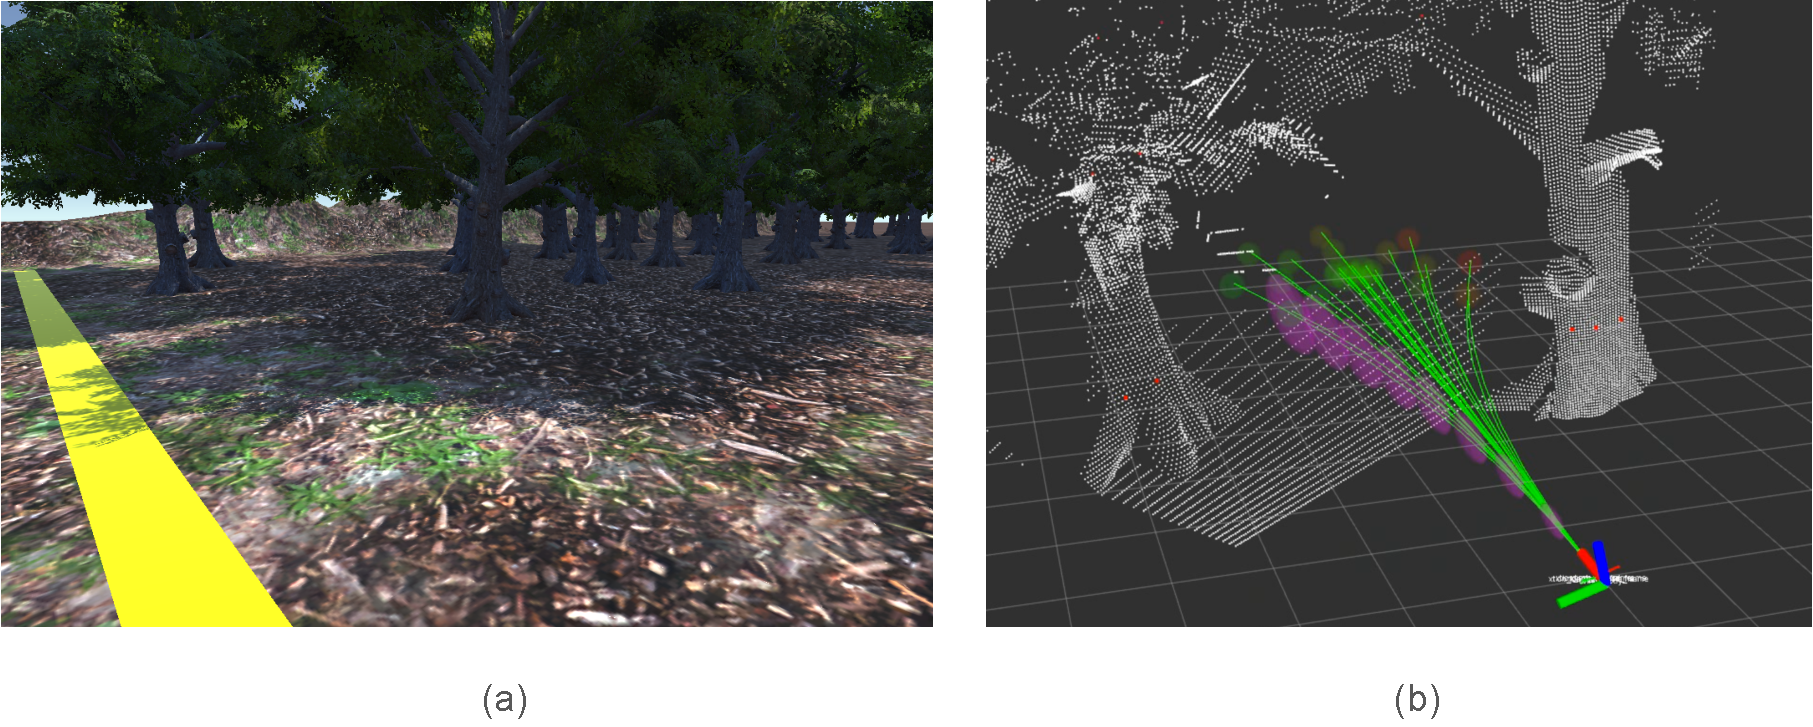
\includegraphics[keepaspectratio=true,scale=0.41]{images/unity_rviz.pdf}
  \captionof{figure}{Screenshots from our race-through-forest simulation environment. (a) Screenshot from Unity of our forest simulation environment. (b) Screenshot from Rviz which shows the evaluation of the 25-trajectory real-time-generated MPC-library.  The chosen trajectory and the $1$-$\sigma$ of the Gaussian distribution over time are visualized for the chosen trajectory.  The small sphere at the end of each trajectory indicates approximated collision probabilities from low to high (green to red), evaluated against the 160x120 depth image point cloud (white) and 100-laser 2-dimensional LIDAR point cloud (red).}\label{success_heatmap}%      only if needed  
\end{center}
To facilitate the comparison study, simulation software was developed to closely mimic the capabilities of our hardware platform for the Draper-MIT DARPA FLA (Fast Lightweight Autonomy) research team.  The sensor configuration includes a depth sensor that provides dense depth information at 160x120 resolution out to a range of 10 meters, with a FOV (field of view) limited to 58 degrees horizontally, 45 degrees vertically.  To complement the range and horizontal field of view limitations of the camera system, a simulated 2D scanning lidar is incorporated to provide range measurements reaching out to 30 meters.  Both depth sensors are simulated at 30 Hz.  Pixhawk software is used to control the attitude and thrust of the quadrotor.

Drake was used to simulate vehicle dynamics using a common quadrotor 12-state nonlinear quadrotor model while Unity (game engine) provides high fidelity simulated perceptual data that includes GPU-based depth images and raycasted 2D laser scans.  The flight controller uses a version of the Pixhawk firmware running in the loop (SITL) that utilizes an EKF over noisy simulated inertial measurements to estimate attitude and attitude rates of the vehicle. We use ROS as the underlying communication and logging layer to tie the various subsystems together and MAVROS is used to send attitude and thrust setpoints to the Pixhawk flight controller software.

\subsection{Experimental setup}

The experiments were carried out in a virtual environment that consists of an artificial forest valley that is 50 meters wide and 160 meters long. The corridor is filled with 53 randomly placed trees whose trunks are roughly 1 meter in diameter and is surrounded by steep, impassable terrain.  SpeedTree was used for the tree geometry and includes simulated wind that articulates the branches and leaves to increase the realism of the perceptual data.

For each experimental trial, the vehicle is started on one side of the forest valley and is commanded to fly at 1.8 meters altitude to a goal on the far end, forcing it to traverse a 150 meter stretch of the obstacle-laden environment.  A timer is started when the vehicle crosses the 5 meter mark and stopped either when a collision occurs or when the 155 meter mark is reached.  If the vehicle is able to navigate the forest without colliding with any of the trees or terrain, the trial is considered a success.  If a collision occurs or if the finish line has not been reached in a predetermined amount of time, the trial is considered a failure.

The experiments were repeated for each algorithm at various target velocities $\{$ 3, 5, 8, 12$\}$ meters per second and with increasing levels of state estimate noise for $x, \dot{x}, y, \dot{y}$. We do not simulate noise in the altitude or in the orientation or angular velocities since these are more easily measurable quantities. To simulate noise that causes position to drift over time, we take the true difference in $x, y$ over a timestep, $\Delta \mathbf{p}_{x,y}(t)$, and add zero-mean Gaussian noise which is scaled linearly with the velocity vector.  The three noise levels we use are $\sigma = \{0, 0.1, 1\}$ which is scaled by $\frac{\sigma}{10}\mathbf{v_{true}}$.  We also add true-mean Gaussian noise to $\dot{x}$ and $\dot{y}$, with standard deviations that are the same as for position noise.  Accordingly we have:
%
\begin{center}
$$\mathbf{p}_{noisy}[i+1] \sim \mathcal{N}(\mathbf{p}_{true}[i+1] -\mathbf{p}_{true}[i] ,\frac{\sigma}{10}\mathbf{v_{true}})$$ 
$$\mathbf{v}_{noisy}[i] \sim \mathcal{N}(\mathbf{v}_{true}[i],\frac{\sigma}{10}\mathbf{v_{true}})$$
\end{center}
%
The total time taken and the trial outcome was recorded for 10 trials at each noise and speed setting.  The results are tabulated in grid form and indicate the path taken through the forest on each trial as well as the overall success rate of each method.

\subsection{Pure pursuit algorithm description}

We compare our method to a typical map-based robotics navigation solution that consists of a global path planner that is paired with a path following algorithm.  The particular implementation we chose functions by maintaining a global probabilistic occupancy grid (Octomap) with a 0.2 meter voxel size into which all incoming depth information is inserted and registered with the current vehicle pose.  At a specified rate, a horizontal slice of the map is extracted and a globally optimal path from the vehicle's position to the goal is computed using Dijkstra's algorithm.  The path planning includes a soft cost on proximity to obstacles to find paths that maintain sufficient clearance.  We then use a pure pursuit algorithm to command a vehicle velocity along the resulting path to the goal.  

This approach has been validated in hardware during experiments in which the quadrotor was commanded to navigate a previously unknown cluttered warehouse environment at speeds ranging from 2.0 m/s to 5.5 m/s to a goal approximately 65 meters from the starting location.  Using this method, we have been able to successfully navigate through 24 randomly configured obstacle courses using a state estimator that fuses measurements from a laser scan matcher with accelerometer and gyroscope data from the Pixhawk's IMU.

\section{Simulation Results and Discussion}

The key metric for our comparison of the three methods is the no-collison success rate of reaching the finish line, and is presented in Figure \ref{success_heatmap}.

The results for the global path planning and following approach show both the limitations on handling higher speed, and on handling higher state estimate noise.  The approach was not able to handle any of the severe noise ($\sigma=1$) for any of the speeds and was only able to reliably reach the goal at 5 m/s and below, with zero or little state estimate noise.  These limits on speed and state estimate noise match well our experimental results in hardware.  Primary inhibiting factors for this approach's success are (i) dependence on a global position estimate, (ii) latency incurred by processing sensor data into a global map, (iii) latency incurred by path planning on the local map, and (iv) neglect of vehicle dynamics, which are increasingly important for obstacle avoidance at higher speeds.

For the deterministic method, the average time to goal on a successful run was faster than the probabilistic method by approximately 14\%.   However, the deterministic nature of the collision checking causes the method to leave little margin for error while navigating around obstacles.  Thus, small inaccuracies in the model or the state estimate can lead to fatal collisions.  

The results for the probabilistic method demonstrate a marked increase in robustness at higher speeds and with the highest of state estimate noise.  The sacrifice in average time to goal is outweighed by the gains in robustness. Since the methods differ only in the way they consider collisions, the results suggest that the probabilistic method is superior.  

Additionally, an important practical consideration is that, given our fast collision probability approximations as presented, the computational costs of both methods are nearly identical, as is displayed in Table 1.  This is a strong argument for replacing deterministic collision checking with fast collision probability approximation in a wide number of scenarios.

\begin{center}
  \includegraphics[keepaspectratio=true,scale=0.55]{images/success_heatmap_3.pdf}
  \captionof{figure}{Comparison summary of number of successful collision-free trials for the different approaches tested in in our simulated quadrotor race through the forest.  Ten trials were run for each of the three approaches, for four different speeds $\{$3, 5, 8, 12$\}$ meters per seconds, and for three different levels of 2-dimensional state estimate noise ($x$-$y$ only, no noise on $z$), $\sigma$=\{0,1,10\} for $\mathbf{p}_{noisy}[i+1] \sim \mathcal{N}(\mathbf{p}_{true}[i+1] -\mathbf{p}_{true}[i] ,\frac{\sigma}{10}\mathbf{v_{true}})$ and $\mathbf{v}_{noisy}[i] \sim \mathcal{N}(\mathbf{v}_{true}[i],\frac{\sigma}{10}\mathbf{v_{true}})$ as described.}\label{success_heatmap}%      only if needed  
\end{center}

%Comparison vs. traditional \cite{director} global-state-estimate-tracking\cite{barry2016}, when increasing noise on local position estimate.

%\begin{center}
%  \includegraphics[keepaspectratio=true,scale=0.55]{images/latencies.png}
%  \captionof{figure}{Comparison summary of number of successful collision-free trials for the different approaches tested in in our simulated quadrotor race through the forest.  Ten trials were run for each of the three approaches, for four different speeds (3, 5, 8, 12 meters / seconds), and for three different noise scalings as described.}\label{success_heatmap}%      only if needed  
%\end{center}

\begin{center}
\label{table_speeds}
\scalebox{0.55}{
  \begin{tabular}{lcccccc}
	 &  \textbf{Deterministic, N=1}  & & \textbf{Probabilistic, N=1}  & &  \textbf{Probabilistic, N=10}& \\ \\ \hline \hline
					&   Average					&  Percentage    &   Average 		 &  Percentage		 &   Average		 &  Percentage		 \\ 
	 Subprocess                				&  				time ($\mu$s) &  	 time (\%)  &   	 time ($\mu$s) &  	 time (\%) &   		 time ($\mu$s) &  	 time (\%) \\ \hline \hline
	\\
	Building kd-tree & 1900 +/- 700 & 51.0  & 2000 +/- 500 & 58.4 & 1900 +/- 400 & 43.0 \\ 
	\\
	Evaluating future positions from real-time \\
	generated 25-trajectory MPC-library & 4 +/- 1 & 0.1 & 4 +/- 1 & 0.1 & 4 +/- 1 & 0.1\\
	\\
	Evaluating collision probabilities with N-nearest \\
	neighbor search on kd-tree & 1800 +/- 800 & 48.3 & 1400 +/- 600 & 40.9 & 2500 +/- 1000 & 56.5 \\
	\\
	Evaluating expected reward, given $R_{nav}$ & 2 +/- 1 & 0.1 & 2 +/- 1 & 0.1 & 2 +/- 1 & 0.0 \\
	\\
	Calculating attitude setpoint for attitude controller & 17 +/- 5 & 0.5 & 17 +/- 5 & 0.5 & 17 +/- 5 & 0.4 \\
	\\
	
  \end{tabular}
}
\captionof{table}{Measured averages and standard deviations of subprocess latencies for our implementations.}
\end{center}

\section{Future Work}


There are several extensions to this line of work that we plan to work on in the near future.  For one, we plan to validate the method in hardware.  Additionally, the highly parallel nature of the fast collision probability approximation algorithm is amenable to data-parallel implementations on a GPU.  We also plan to expand on the MPC-library approach, including true 3D flight, increased variety of maneuvers, and analysis of the accuracy of the model approximation.  We also plan to characterize the performance of the collision probability approximation with more elaborate global navigation functions.

%\section{Graveyard}
%
%
%\subsubsection{Limitations of depth-image-only probabilistic collision approximation}
%
%Although using the most recent depth image as the only world geometry data enables very fast probabilistic collision-checking, there are limitations imposed by the sensor FOV, range, and lack of memory used.  If the robot point is out of the depth image's pixel bounds, or the robot point is behind the camera, then a probability of collision in the unknown $P(\text{Collision in Unknown})$ must be assigned.  The conservative approach is to assign this to 1, while the aggressive approach is to assign this to 0.  Since turning into the unknown is certainly better than flying into a known wall, but much riskier than going into a known open area, something between 0 and 1 is probably appropriate.  A supervised-learning approach which trains a model of collision with the unknown through simulation could be used to better estimate this probability. (Richter 2015).
%
%It should also be noted that Gaussian noise on depth points is certainly an imperfect approximation of depth image noise (particularly for passive mono/stereo depth images, where the failure modes are more binary ``didn't see the dark object'' rather than Gaussian decay.  The Gaussian-noise approximation, however, is preferable to only deterministic collision-checking, and future work may investigate probabilistic formulations more suited for passive camera depth images.  It is also noted that a single point in a Cartesian frame is an imperfect representation of the frustum of a depth image pixel, but it is an approximation and allows simple computational treatment.
%
%
%\subsubsection{Alternative using a history of depth images, or a local map}
%
%Two methods for incorporating histories of depth images are considered below.  Even without considering history, the global navigation function $R_{nav}$ can be responsible for remembering history and guiding the robot away from obstacles outside of its instantaneous depth image FOV.
%
%Rather than only consider the instantaneous depth image, the last $N$ depth images could be used, and the independence approximation (Equation \ref{prob_whole_trajectory}) can just be extended to assume independence between depth images.  The calculation is identical, except the initial position $\textbf{p}_0$ for previous depth images is set to be the estimate of the position traveled during the $\Delta t$ passed since the timestamp of that depth image.  Alternatively, a $k$-$d$-tree can hold all the points form the last $N$ depth images.
%
%\begin{thebibliography}{1}
%\bibitem {clar:eke}
%Clarke, F., Ekeland, I.:
%Nonlinear oscillations and boundary-value problems for
%Hamiltonian systems.
%Arch. Rat. Mech. Anal. {\bfseries 78} (1982) 315--333
%\end{thebibliography}

\bibliography{wafr-bib}
\bibliographystyle{splncs}


\end{document}

